\documentclass[12pt]{article}
%% arXiv paper template by Flip Tanedo
%% last updated: Dec 2016



%%%%%%%%%%%%%%%%%%%%%%%%%%%%%
%%%  THE USUAL PACKAGES  %%%%
%%%%%%%%%%%%%%%%%%%%%%%%%%%%%

\usepackage{amsmath}
\usepackage{amssymb}
\usepackage{amsfonts}
\usepackage{graphicx}
\usepackage{xcolor}
\usepackage{nopageno}
\usepackage{enumerate}
\usepackage{parskip}


\renewcommand{\thesection}{}
\renewcommand{\thesubsection}{\arabic{subsection}}

%%%%%%%%%%%%%%%%%%%%%%%%%%%%%%%%%%%%%%%%%%%%%%%
%%%  PAGE FORMATTING and (RE)NEW COMMANDS  %%%%
%%%%%%%%%%%%%%%%%%%%%%%%%%%%%%%%%%%%%%%%%%%%%%%

\usepackage[margin=2cm]{geometry}   % reasonable margins

\graphicspath{{figures/}}	        % set directory for figures

% for capitalized things
\newcommand{\acro}[1]{\textsc{\MakeLowercase{#1}}}    

\numberwithin{equation}{section}    % set equation numbering
\renewcommand{\tilde}{\widetilde}   % tilde over characters
\renewcommand{\vec}[1]{\mathbf{#1}} % vectors are boldface

\newcommand{\dbar}{d\mkern-6mu\mathchar'26}    % for d/2pi
\newcommand{\ket}[1]{\left|#1\right\rangle}    % <#1|
\newcommand{\bra}[1]{\left\langle#1\right|}    % |#1>
\newcommand{\Xmark}{\text{\sffamily X}}        % cross out

\let\olditemize\itemize
\renewcommand{\itemize}{
  \olditemize
  \setlength{\itemsep}{1pt}
  \setlength{\parskip}{0pt}
  \setlength{\parsep}{0pt}
}


% Commands for temporary comments
\newcommand{\comment}[2]{\textcolor{red}{[\textbf{#1} #2]}}
\newcommand{\flip}[1]{{\color{red} [\textbf{Flip}: {#1}]}}
\newcommand{\email}[1]{\texttt{\href{mailto:#1}{#1}}}

\newenvironment{institutions}[1][2em]{\begin{list}{}{\setlength\leftmargin{#1}\setlength\rightmargin{#1}}\item[]}{\end{list}}


\usepackage{fancyhdr}		% to put preprint number



% Commands for listings package
%\usepackage{listings}      % \begin{lstlisting}, for code
%
% \lstset{basicstyle=\ttfamily\footnotesize,breaklines=true}
%    sets style to small true-type



%%%%%%%%%%%%%%%%%%%
%%%  HYPERREF  %%%%
%%%%%%%%%%%%%%%%%%%

%% This package has to be at the end; can lead to conflicts
\usepackage{microtype}
\usepackage[
	colorlinks=true,
	citecolor=black,
	linkcolor=black,
	urlcolor=green!50!black,
	hypertexnames=false]{hyperref}





\begin{document}


\begin{center}

    {\Large \textsc{Short HW 2}:
    \textbf{Momentum Flow}}
    
\end{center}

\vskip .4cm

\noindent
\begin{tabular*}{\textwidth}{rl}
	\textsc{Course:}& Physics 165, \emph{Introduction to Particle Physics} (2018)
	\\
	\textsc{Instructor:}& Prof. Flip Tanedo (\email{flip.tanedo@ucr.edu})
	\\
	\textsc{Due by:}& \textbf{Thursday}, January 18
\end{tabular*}

\noindent
Note that this short assignment is due in class on Thursday. You have only \emph{two days} to do it. This should be quick, I recommend doing it right after class on Tuesday.

\subsection{Total Momentum Conservation for  a $2\to 3$ process}

In class we drew the following diagram for $e^+ e^- \to 3\gamma$. 

\begin{center}
	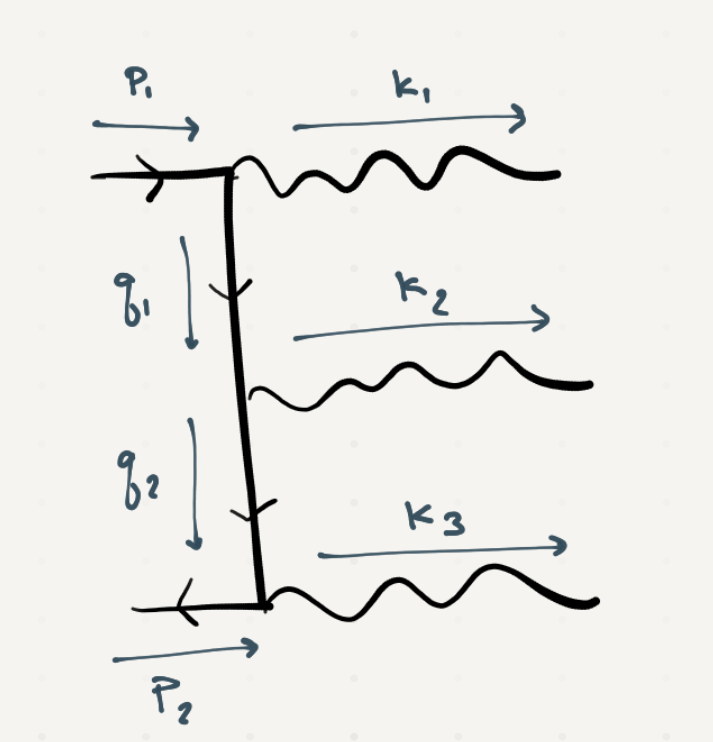
\includegraphics[width=.3\textwidth]{HW2a.png}
\end{center}
Using the conservation of four-momentum at each vertex, show that the total four-momentum is conserved. That is, prove:
\begin{align}
	(p_1 + p_2)^\mu = (k_1 + k_2 + k_3)^\mu \ .
\end{align}
\textsc{Hint:} Start by writing the conservation of four-momentum at each vertex. Those are three equations
%\footnote{...well, 3$\times$4 equations if you count each component separately...} 
with unspecified $q_1^\mu$ and $q_2^\mu$. Use two equations to determine what these virtual momenta are, then plug them into the last equation to prove the above relation.


\subsection{Kinematics}

I totally screwed up on Long Homework 1. $\mu \to e \gamma$ is possible kinematically, though not dynamically in any model we have seen thus far. Ignoring what the Feynman diagram, work out what the magnitude of the 3-momentum of the $\gamma$ is in the muon rest frame. If you haven't turned it in, you should put this in your Long Homework 1 and submit it on Thursday. If you have turned it in, submit it with this Short Homework 2 and I'll grade it accordingly.


\subsection{Read the weekly homework}

Before class on Thursday, go over the weekly (``long'') homework assignment due on January 23. Write out one question that you would like to have answered on Thursday. Ideally it would be about the topics of in the homework. 


\end{document}